% По умолчанию используется шрифт 14 размера. Если нужен 12-й шрифт, уберите опцию [14pt]
\documentclass[14pt]{matmex-diploma-custom}
\usepackage{graphicx}
\usepackage{xcolor}
\usepackage{minted}
\usepackage{amsmath,amssymb,amsfonts,amsthm}
\usepackage{multicol}
\usepackage{mathtools}
\usepackage[title]{appendix}
\usepackage{subfiles}

\newtheorem{thm}{Теорема}[subsection]
\newtheorem{defn}{Определение}[subsection]
\newtheorem{exmp}{Пример}

\begin{document}
\filltitle{ru}{
    chair              = {Математическое обеспечение и администрирование \\ информационных систем \\ \vspace{5mm} Системное программирование},
    title              = {Реализация алгоритма построения представления группы по машине Тьюринга},
    type               = {bachelor},
    position           = {студента},
    group              = 443,
    author             = {Шамрай Максим Борисович},
    supervisorPosition = {к.~ф.-м.~н., доцент},
    supervisor         = {Григорьев С.\,В.},
    reviewerPosition   = {ведущий инженер ООО "Ланит-Терком"},
    reviewer           = {Смирнов К.\,К.},
    chairHeadPosition  = {д.\,ф.-м.\,н., профессор},
    chairHead          = {Терехов А.\,Н.}
    }
    
\filltitle{en}{
    type               = {bachelor},
    chair              = {Software and Administration of Information Systems \\ \vspace{5mm} Software Engineering},
    title              = {Implementation of the algorithm for constructing a finitely presented group by a Turing machine},
    author             = {Maksim Shamrai},
    supervisorPosition = {Assistant Professor},
    supervisor         = {Semyon Grigorev},
    reviewerPosition   = {Senior engineer at Lanit-Tercom LLC},
    reviewer           = {Kirill Smirnov},
    chairHeadPosition  = {Professor},
    chairHead          = {Andrey Terekhov}
}
\maketitle
\tableofcontents

\section*{Введение}
Формальные языки являются теоретическим основанием системного программирования, а именно
разработки трансляторов и статических анализаторов посредством 
лексического, синтаксического и семантического анализов. Теория формальных языков начала свое активное развитие в 50-х годах прошлого века \cite{chomsky1, chomsky2}.
За это время она нашла свое применение не только в областях связанных непосредственно с
системным программированием, но, кроме прочего, и в анализе графовых моделей данных \cite{Hellings2015QueryingFP, Azimov2017ContextfreePQ}, которые
применяются, например, в биоинформатике и социальных сетях. 

Развитие влечет за собой новые теоретические проблемы и неразрешенные задачи. 
В качестве примера приведем проблему связанную с появлением таких классов языков, как конъюнктивные \cite{ConjGrammars} и булевы \cite{BoolGrammars}.
Она касается
ограничений соответствующих грамматик. Ограничения выразительной силы обычных контекстно-свободных грамматик
известны довольно хорошо. Существуют прямые методы доказательства непредставимости
определенных языков, таких как лемма накачки и ее
варианты, которые показывают, что некоторые языки не могут быть заданы
 контекстно-свободной грамматикой. Напротив, нет методов доказывания
непредставимости языков булевыми грамматиками, и это главный пробел в
знаниях этих грамматик. Точно так же такие методы неизвестны
и для конъюнктивных грамматик \cite{OKHOTIN201327}.

В последнее время наблюдается тенденция смещения направления методов изучения формальных языков. Наряду с классическими комбинаторными исследователи начинают все активней применять методы из других разделов математики.
Одно из возможных направлений --- исследование формальных языков с помощью обращения 
к теоретико-групповому аппарату.

Стоит отметить, что когда говорят о группах в языковом контексте, часто имеют в виду изоморфное представление группы, определение которого будет представлено далее.
По описанию представления группы можно естественным образом задать формальный язык, однако в обратную сторону --- по грамматике построить группу --- задача нетривиальная, то есть не существует простого способа построения представления группы по формальному языку.
Для этого проводятся сложные математические преобразования распознающей язык машины Тьюринга, и
производить их с помощью ручки и бумаги не является целесообразным, а изучать
групповые свойства языков выглядит довольно перспективным направлением исследований \cite{Sapir, SpaceFunc}.

Таким образом, актуальной является задача алгоритмизации построения представления группы по машине Тьюринга, так как исследования языков в этом направлении представляют особый интерес. Также в данной работе будут затронуты только контекстно-свободные языки, так как они одни из самых хорошо изученных и востребованных.

\subsection*{Постановка задачи}
Целью данной работы является предоставление исследователям возможности ставить вычислительные эксперименты по преобразованию формального языка в соответствующее представление группы.

Достижение поставленной цели обеспечивается решением следующих задач:
    \begin{enumerate}
    \item Реализовать алгоритм преобразования контекстно-свободной грамматики в машину Тьюринга.
    \item Разработать алгоритм построения представления группы по машине Тьюринга.
    \item Разработать интерпретаторы промежуточных машин для проверки эквивалентности преобразований в контексте сохранения распознаваемого языка.
    \item Провести эксперименты.
\end{enumerate}

\section{Обзор}
В данном разделе приведены определения и теоремы, используемые в данной работе, рассмотрена связь между формальными языками и группами, а также рассмотрен формальный алгоритм построения представления группы по машине Тьюринга, предложенный в статье \cite{Sapir}.

\subsection{Формальные языки}
В этой работе используется стандартные определения теории формальных языков, которые можно увидеть,
например, в работах Хомского~\cite{chomsky1, chomsky2}. 
Далее будут рассмотрены основные определения, которые используется в данной работе. 

\begin{defn}
В классической формализации формальная грамматика G может быть представлена 
в виде четырехместного кортежа $G = (\Sigma, N, R, S)$, который состоит из следующих компонентов:
\begin{itemize}
    \item Конечное множество $\Sigma$ терминальных символов.
    \item Конечное множество $N$ нетерминальных символов, которое не пересекается с $\Sigma$.
    \item Конечное множество $R$ правил вывода, каждое правило представимо в виде: 
    $(\Sigma \cup N)^{*}N(\Sigma \cup N)^{*} \to (\Sigma \cup N)^{*}$
    \item $S \in N$ --- стартовый нетерминал.
\end{itemize}
\end{defn}

\begin{defn}
Контекстно-свободная грамматика является формальной грамматикой
(тип 2 в иерархии Хомского), в которой левые части всех правил вывода 
являются единичными нетерминалами. 
\end{defn}

Примером правила контекстно-свободной грамматики может служить $A \to X_1 \dots X_l$.
Оно означает, что каждое слово, представимое в виде конкатенации $X_1 \dots X_l$, 
обладает свойством $A$.

Определим автомат с магазинной памятью, который нам пригодится в алгоритме
построения машины Тьюринга по контекстно-свободной грамматике. Также ниже приведена теорема, благодаря которой можно
утверждать, что этот алгоритм строит машины Тьюринга, которые распознают в точности контекстно-свободные
языки.

\begin{defn}
Автомат с магазинной памятью --- это конечный автомат с дополнительным хранилищем стека, 
переходы которого основаны не только на входе и текущем состоянии, но также и на символах на стеке. 
Формальное определение выглядит как кортеж из семи состовляющих:
$M=(Q,\Sigma ,\Gamma ,\delta ,q_{0},Z,F)$, где
\begin{itemize}
    \item $Q$ --- конечное множество состояний.
    \item $\Sigma$ --- конечный алфавит входных символов. 
    \item $\Gamma$ --- конечный алфавит символов на стеке.
    \item $\delta \subset (Q \times (\Sigma \cup \{\varepsilon \})\times \Gamma) \times (Q\times \Gamma^{*}))$ --- конечное множество переходов.
    \item $q_{0}\in Q$ --- начальное состояние.
    \item $Z\in \Gamma$ --- начальный символ стека.
    \item $F\subseteq Q$ --- множество конечных состояний.
\end{itemize}
\end{defn}

\begin{thm} \label{thmpda}
Множество языков, допускаемых автоматами с магазинной памятью, совпадает с множеством контекстно-свободных языков \cite{hopcroft2013introduction}.
\end{thm}

\subsection{Основные сведения из теории групп}

В этом разделе даны определения свободной группе, представлению группы и нескольким базовым определениям и теоремам приводящих к ним. Все описанные в этом
разделе определения и теоремы можно найти в книге А. Ю. Ольшанского~\cite{geomTheoryGroup}.

\begin{defn}
Множество G с заданной на нем операцией ($ \cdot $) называется группой, если верно следующее:
\begin{itemize}
\item $\forall a, b, c \in G, (a \cdot b) \cdot c = a \cdot (b \cdot c)$
\item $\exists e \in G :$ $\forall a, a \cdot e = e \cdot a = a$
\item $\forall a \in G$ $\exists a^{-1} \in G :  a \cdot a^{-1} = a^{-1} \cdot a = e$
\end{itemize}
\end{defn}

В теории групп смежные классы разделяются в соответствии с положением элемента группы
на правый и левый классы. 
Например, левый смежный класс может быть определен как $aH = \{ah: h \in H \}$,
где $ a \in G $, $ H $ --- подгруппа в $G$.
Подгруппа $ H $ группы $ G $ называется нормальной, если для всех
элементов $ a $ из $ G $ соответствующие левые и правые смежные классы равны,
то есть $ aH = Ha $. Кроме того, смежные классы $ H $ в $ G $ образуют группу, которая
называется фактор-группой.

Нормальное замыкание $ S^G $ подмножества $ S $ группы $ G $ является наименьшей нормальной подгруппой
группы $ G $, которая содержит подмножество $ S $.
\begin{equation}
    S^G = \{ gsg^{-1} : g \in G,\, s \in S \}
\end{equation}

\begin{thm}[Теорема о гомоморфизме] \label{gomomorphThm}
Следующий результат является одним из основополагающих результатов в теории групп.
Если $ \phi: G \to H $ является гомоморфизмом, то $ Im (\phi) \cong G/Ker (\phi) $.
\end{thm}

Пусть $A$ --- произвольное множество символов, тогда $ A^{-1} = \{a^{-1}: a \in A\} $ и $ A \cup A^{-1} $ --- групповой алфавит.
$ \omega $ --- слово в алфавите $ A \cup A^{-1} $, если $\omega = a_1 \dots a_n$,
где $ a_i \in A \cup A^{-1}$ $\forall i$ от $1$ до $n$.
Слово сократимо, если существует $ i $, для которого буквы $ x_i $ и $ x_{i + 1} $ взаимно обратны.

\begin{defn}
Множество $ G (A) $ всех несократимых слов в алфавите $ A \cup A^{-1} $
является группой для операции конкатенации с последующим сокращением и называется свободной группой.
\end{defn}

Поскольку для любой группы с произвольным множеством образующих $ \{g_i \}_{i \in I} $ существует
сюръективный гомоморфизм $ \phi: G (A) \to G $ такой, что $ \phi (a_i) = g_i $,
где $ \{a_i \}_{i \in I} = A $ и $i \in I$. Итак, применяя теорему о гомоморфизме (см. теорему ~\ref{gomomorphThm}), получаем изоморфную фактор группу свободной группы по ядру гомоморфизма:
\begin{equation} \label{eq:isomorph}
  G \cong G (A) / Ker (\phi)  
\end{equation}

Так как по любой нормальной подгруппе возможно определить фактор группу, значит интересна возможность определения каждой группы
как фактор группы свободной группы по некоторой нормальной ее подгруппе.
В связи с этим интересны способы задания нормальной подгруппы в свободной группе, то есть способы задания ядра гомоморфизма из (\ref{eq:isomorph}).

Чтобы определить отношение эквивалентности в словах свободной группы $G(A)$, необходимо описать элементарные преобразования слов, которые не меняются
смежный класс слова в нормальном замыкании $ R^{G (A)} $, где $ R $ является подмножеством в $ G (A) $, следующим образом:
\begin{enumerate}
\item Сокращение.
\item Замена слова $\omega = \omega_1 r^{\pm} \omega_2$, где $r \in R$, словом $\omega_1 \omega_2$ и наоборот.
\end{enumerate}

Если возможно привести слова $ \omega_1 $ и $ \omega_2 $ друг к
другу с помощью этих преобразований, то можно утверждать, что они эквивалентны.

\begin{defn}
Множество отношений $ \{r = 1: r \in R \} $ называется определяющим для группы
$ G = \langle g_i \rangle $, если любое другое отношение между
$ g_i $ получается из системы $ \{r = 1: r \in R \} $. Если множество отношений
$ \{r = 1: r \in R \} $ является определяющим для группы $ G $, тогда $ G \cong G (A)/R^{G (A)} $
и тогда можно сказать, что $ G $ имеет групповое представление $ \langle A ~|~ R \rangle $.
Для обозначения этого пишут $G = \langle A ~|~ R \rangle $.
\end{defn}

Таким образом, было дано определение представлению группы, которое является ключевым в данной работе. 

\subsection{Связь формальных языков с группами}

Рассмотрим связь между формальными языками и группами. 
Пусть $\Sigma$ --- конечный алфавит букв, $(\cdot)$ --- конкатенация двух слов, 
и $\varepsilon$ --- пустое слово.
Тогда 
\begin{itemize}
    \item $(\Sigma^+, \cdot)$ --- свободная полугруппа.
    \item $(\Sigma^*, \cdot, \varepsilon)$ --- свободный моноид.
    \item $((\Sigma \cup \Sigma^{-1})^*, \cdot, \varepsilon)$ --- свободная группа.
\end{itemize}
 
 Действительно, так как для 
полугруппы достаточно, чтобы групповая операция была ассоциативная
$$\forall a, b, c \in \Sigma^+, a(bc)=(ab)c$$
, моноиду еще необходим нейтральный элемент 
$$\forall a \in \Sigma^*, a\varepsilon=\varepsilon a = a$$
, и группе не хватает лишь обратных элементов
$$\forall a \in (\Sigma \cup \Sigma^{-1})^* \, 
\exists a^{-1} \in (\Sigma \cup \Sigma^{-1})^* : a \cdot a^{-1} = a^{-1} \cdot a = \varepsilon$$

Кроме этой очевидной связи, в теории групп существует понятие проблемы слов группы,
которое может быть сформулировано следующим образом. 

\begin{defn}
Проблема слов для конечно порожденной группы $G$ --- это алгоритмическая задача определения, 
представляют ли два слова, состоящие из порождающих, один и тот же элемент. Часто ее сводят к равенству слов единице, что эквивалентно.
\end{defn}

Итак, если $A$ --- конечное множество образующих для $G$, а $A^{-1}$ --- множество его инверсий, 
то проблема слов --- это проблема принадлежности для множества слов над алфавитом 
$\Sigma=A \cup A^{-1}$ групповой единице при отображении естественным гомоморфизмом
$\phi : \Sigma^* \to G$. 

Множество таких слов можно записать следующим образом (см. рис. \ref{fig:word_problem}):
$$W(G) = \phi^{-1}(1) = 
\{ \omega \in \Sigma^* : \phi(\omega) = 1 \}$$

\begin{figure}[H]
\centering
  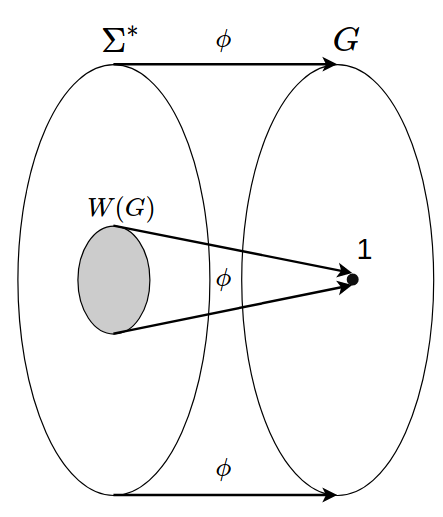
\includegraphics[width=0.5\linewidth]{pics/3.png}
  \caption{Проблема слов группы}
  \label{fig:word_problem}
\end{figure}

Для проблемы слов группы уже доказан ряд утверждений, которые показывают, что
алгебраические свойства групп соответствуют свойствам формальных языков. 
Например, для конечно порожденной группы $G$ верно следующее:
\begin{itemize}
    \item Проблема слов для $G$ разрешима $\iff W(G)$ --- рекурсивный язык. 
    \item $W(G)$ -- регулярный язык $\iff G$ --- конечна \cite{Anisimov}.
    \item $W(G)$ -- контекстно-свободный язык $\iff \exists H < G$ --- свободная подгруппа конечного индекса \cite{Muller}.
\end{itemize}

\subsection{Алгоритм построения представления группы}

Описанная в этом разделе статья посвящена исследованию связей
между асимптотическими функциями групп и вычислительной сложностью~\cite{Sapir}.
В частности, авторы показывают, как построить конечно-представленную группу
с NP-полной проблемой слова. Для этого они доказывают несколько теорем,
которые и будут представлены в этом разделе.

\subsubsection{Машина Тьюринга}

Сапир, Биргет и Рипс в своей работе \cite{Sapir} используют следующую нотацию машины Тьюринга.

\begin{defn} \label{tm}
Машина Тьюринга имеет $ k $ лент и $ k $ голов и может быть описана как шестиместный кортеж:
$M = \langle X, \Gamma, Q, \Theta, \overline{s_1}, \overline{s_0} \rangle$,
где
\begin{itemize}
    \item $X$ --- входной алфавит.
    \item $\Gamma$ --- алфавит лент.
    \item $Q = \cup_{i=1}^k Q_i$ --- множество состояний голов на лентах машины.
    \item $\Theta$ --- множество команд машины.
    \item $\overline{s_1}$ --- k-вектор начальных состояний машины.
    \item $\overline{s_0}$ --- k-вектор конечных состояний машины.
\end{itemize}
\end{defn}

Кроме этого, авторы вводят специальные обозначения $\alpha$ и $\omega$ для крайних левых и правых ячеек соответственно и предполагают, что самая левая (самая правая) ячейка на каждой ленте --- это всегда
$ \alpha $ ($ \omega $). Тем не менее, когда они говорят о слове, записанном на ленте,
они на самом деле не включают эти ячейки в состояние головы, и в каждый момент времени голова
наблюдает только две ячейки на каждой ленте.

Конфигурация ленты --- это слово $ \alpha u q v \omega $, где $ q $ --- текущее состояние головы на ленте, 
$u$ ($ v $) --- слово слева (справа) от головы. 
Входная конфигурация --- это конфигурация, в которой слово, записанное на первой ленте, из
$X^+$, все остальные ленты пусты, голова видит правый маркер $\omega$, и состояния формируются
начальный вектор $s_1$. Принимающая конфигурация --- это любая конфигурация, в которой вектор состояния
$s_0$. 

Команда машины Тьюринга определяется состояниями голов и некоторыми из
$ 2k $ букв, наблюдаемых головами.
В результате команды возможно заменить какие-то из этих $ 2k $ букв другими буквами,
добавить новые ячейки на ленты, удалить ячейки на лентах и переместить
голову на одну ячейку влево (вправо) на лентах.
Единственным ограничением является то, что машина может вставлять или удалять ячейки на ленте,
но непосредственно перед знаком $ \omega $, и ячейка не может быть вставлена слева (справа) от
$ \alpha $ ($ \omega $), и эти крайние маркеры нельзя удалять.

Далее в качестве примера приведены команды одноленточной машины Тьюринга, 
которые в результате заменяют \eqref{eqreplace},
вставляют \eqref{eqinsert}, перемещают влево \eqref{eqmove} и удаляют ячейки \eqref{eqdelete}.

\begin{equation}
    u q v \to u' q' v' \label{eqreplace}
\end{equation}
\begin{equation}
    q \omega \to u q' \omega \label{eqinsert}
\end{equation}
\begin{equation}
    u q \to q' u \label{eqmove}
\end{equation}
\begin{equation}
    u q \omega \to q' \omega \label{eqdelete}
\end{equation}
где $u$, $v$, $u^{'}$, $v^{'}$ --- символы алфавита ленты. 

\subsubsection{Симметричные машины Тьюринга}

В дальнейших теоремах будет использоваться класс машин Тьюринга,
называемый симметричными машинами Тьюринга. Дадим определения, которые можно увидеть, 
например, в \cite{symTM}.

\begin{defn}
Машина Тьюринга M симметрична, если для каждой команды в наборе команд существует
обратная ей команда. То есть для любой команды $ u q v \to u' q' v'$ из множества команд 
M в нем также есть команда $ u' q' v' \to u q v $.
\end{defn}

\begin{defn}
Симметризация машины Тьюринга M --- это машина $M^{sym}$, полученная из M путем добавления обратной 
команды $\tau^{-1}$ в множество команд для каждой команды $\tau$ из M.
\end{defn}

\begin{defn}
Машина Тьюринга M подтвергается симметризации тогда и только тогда, 
когда M и $M^{sym}$ эквивалентны (т. е. они принимают один и тот же язык).
\end{defn}

Следующая теорема является фундаментальной в изучении проблемы слов и была получена 
Э. Постом и А. А. Марковым независимо друг от друга в 1947 году.

\begin{thm} \label{symDetTm}
Каждая детерминированная машина Тьюринга подтвергается симметризации. 
С другой стороны, не все недетерминированные машины Тьюринга могут быть симметризованы.
\end{thm}

\subsubsection{S-машина}

Далее перейдем к последнему определению, введенному авторами, системы переписывания 
под названием S-машина, которая играет ключевую роль в построении представления группы.

\begin{defn}
Пусть $ n $ --- натуральное число.
Аппаратное обеспечение (hardware) S-машины --- это пара $ (Y, Q) $, где
\begin{itemize}
    \item $ Y $ --- это $ n $-вектор, где $ Y_i $ --- алфавит на ленте i.
    \item $ Q $ является $ (n + 1) $-вектором непересекающихся множеств $ Q_i $, элементы которых 
    являются состояниями соответствующей ленты i.
\end{itemize}
Множества элементов $ Q $ и $ Y $ также не пересекаются.
\end{defn}

С каждым аппаратным обеспечением $ S = (Y, Q) $ можно связать язык допустимых слов
$ L (S) = Q_1F(Y_1) Q_2 \dots F (Y_n) Q_{n + 1} $, где $ F (Y_j) $ --- язык
всех сокращенных групповых слов в алфавите $ Y_j \cup Y_j^{-1} $.

Правила перезаписи или S-правила имеют следующую форму:
$ [U_1 \to V_1, \dots, U_m \to V_m] $
где выполняются следующие условия:
\begin{enumerate}
    \item Каждый $ U_i $ является подсловом допустимого слова, начинающимся с символа $ Q_l $ и заканчивающейся буквой $ Q_r $.
    \item Если $i < j$, то $r(i) < l(j)$.
    \item Каждый $ V_i $ также является подсловом допустимого слова, чьи состояния $Q$ 
    принадлежат $ Q_{l(i)} \cup \dots \cup Q_{r(i)} $ и которое содержит по состоянию из $Q_l$ и из $Q_r$.
    \item Буквы ленты не вставляются слева от состояний $ Q_1 $ и справа от состояний $ Q_{n + 1} $.
\end{enumerate}

Применить S-правило к слову $ W $ означает заменить одновременно
подслова $ U_i $ на подслова $ V_i $, $ i = 1, \dots, m $. 
После каждого применения правила переписывания, слово автоматически сокращается.

Например, если к слову $ q_1 a a q_2 b q_3 $ применить S-правило
$\newline
[q_1 \to p_1 a^{-1}, q_2 b q_3 \to a^{-1} p_2 b' q_3]$,
где $q_i \in Q_i$, $p_i \in Q_i$, $a \in Y_1$, $b, b' \in Y_2$, то результат
применения этого правила --- $ p_1 p_2 b' q_3 $.

Кроме того, с каждым S-правилом $ \tau $ нам нужно связать обратное 
S-правило $ \tau^{-1} $ следующим образом:
если
$\\ \tau = [U_1 \to x_1 V_1 y_1, \dots, U_m \to x_m V_m y_m]$
, тогда
$\\ \tau^{-1} = [V_1 \to x_1^{-1} U_1 y_1^{-1}, \dots, V_m \to x_m^{-1} U_m y_m^{-1}]$

Стоит отметить, что на протяжении всей своей работы авторы предполагают, что
S-машина симметрична; то есть, если S-машина содержит
правило переписывания $ \tau $, оно также содержит правило $ \tau^{-1} $.

\subsubsection{Используемые в построении теоремы}

Итак, ранее были даны все необходимые определения, и далее будут представлены теормемы их связывающие,
на доказательствах которых и основан наш алгоритм построения представления группы по машине Тьюринга.

Так, например, следующая теорема утверждает, что для любой машины Тьюринга $M$ (в том числе недетерминированной) существует эквивалентная ей симметричная машина Тьюринга, но которая не является ее симметризацией $M^{sym}$. То есть для построения эквиалентной симметричной машины Тьюринга для любой машины Тьюринга производятся более сложные построения, чем обычная симметризация в теореме \ref{symDetTm}. Действительно, 
первыми аналогичную теорему доказали Г. Р. Леви и Х. Пападимитриу~\cite{LEWIS1982161}. 
Авторы рассматриваемой нами статьи модифицируют построение такой машины из~\cite{symTM}.

\begin{thm} \label{symthm}
Для любой машины Тьюринга $M$, распознающей язык $L$, существует
Машина Тьюринга $M'$ со следующими свойствами:
\begin{enumerate}
    \item Язык, который распознает $M'$ --- это $L$.
    \item $M'$ симметрична.
    \item Машина принимает слово только тогда, когда все ленты пусты.
    \item Любая команда $M'$ или ее обратная имеет одну из следующих форм для некоторого i:
    \begin{align}
        \{q_1\omega \to q_1'\omega, ..., q_{i−1}\omega \to q′_{i−1}\omega, 
        a q_i\omega \to q′_i\omega, q_{i+1}\omega \to q′_{i+1}\omega, ...\} \label{symType1} \\
        \{q_1\omega \to q_1'\omega, ..., q_{i−1}\omega \to q′_{i−1}\omega, 
        \alpha q_i\omega \to \alpha q′_i\omega, q_{i+1}\omega \to q′_{i+1}\omega, ...\} \label{symType2}
    \end{align}
    где $a$ принадлежит ленточному алфавиту ленты $i$, а $q_j, q′_j$ являются состояниями ленты $j$.
    \item Буквы, используемые на разных лентах, включая состояния, принадлежат не пересекающимся алфавитам.
\end{enumerate}
\end{thm}

Отметим, что симметричные машины Тьюринга более похожи на группы, чем обычные, из-за возможности обратных вычислений, которые возможны в группах.
Доказательство этой теоремы позволяет построить симметричную машину Тьюринга,
сохраняя распознаваемый язык оригинальной машины.

На следующем этапе авторы предлагают построить S-машину из симметричной
Машина Тьюринга для достижения еще большего сходства с группами.
Существует «естественный» способ преобразования машины Тьюринга в S-машину.
Для этого возьмем машину Тьюринга $ M $, удовлетворяющую всем условиям теоремы \ref{symthm},
объединим все ленты машины $ M $ и заменим каждую команду
$$ a q \omega \to q' \omega $$
на 
$$ q \omega \to a^{- 1} \omega $$
, таким образом команды $ M $ становятся S-правилами.
К сожалению, S-машина, построенная таким образом, не наследует большинство
свойств оригинальной машины $M$. Это происходит потому, что алфавит S-машины
содержит символы обратного алфавита. Следовательно, получается, что
с одной стороны, S-машины гораздо лучше подходят для имитации своей работы групповыми отношениями, 
чем обычные машины Тьюринга, так как S-машина может работать с символами обратного алфавита (и, более того, S-машины сами рассматриваются в \cite{alex2004groups} 
как HNN-расширения свободной группы с базисом $Y \cup Q$), а с другой стороны, когда симметричная
машина Тьюринга начинает работать как S-машина, число принятых слов может бесконтрольно увеличиваться, так как существует возможность распознавать отрицательные слова. 
Из этого становится очевидным, что для сохранения распознаваемого языка необходимо проводить
дополнительные построения.

Прежде чем приступить к построению S-машины, авторы делают следующие переименования.
Для каждого $ q \in Q $ слово $ q \omega $ обозначается через $ F_q $, а левый маркер
на ленте $ \# i $ заменяют на $ E_i $. После переименования правила симметричной машины Тьюринга 
или их обратные имеют одну из следующих форм для некоторого $i$:

\begin{equation} \label{21}
    \{F_{q_1} \to F_{q'_1}}, \dots , aF_{q_i} \to F_{q'_i}, \dots , F_{q_k} \to F_{q'_k}\}
\end{equation}
, где $a \in Y$, или
\begin{equation} \label{22}
    \{F_{q_1} \to F_{q'_1}}, \dots , E_i F_{q_i} \to E_i F_{q'_i}, \dots , F_{q_k} \to F_{q'_k}\}
\end{equation}

Кроме того, для любой конфигурации $ C = (E_1 u_1 F_{q_1}, ..., E_k u_k F_{q_k}) $
машины $ M $, они вводят
значение $ \sigma (C) $, которое является допустимым словом для $S(M)$:

\begin{array}{lCr}
E(0)\alpha^n x(0)F(0) \nonumber \\
E(1)u_1x(1)F_{q_1}(1)E'(1)p(1)\delta^{||u_1||}q(1)r(1)s(1)t(1) \nonumber \\
\overline{p}(1)\overline{q}(1)\overline{r}(1)\overline{s}(1)
\overline{t}(1)F'_{q_1}(1) \nonumber \\
... \nonumber \\
E(k)u_k x(k)F_{q_k}(k)E'(k)p(k)\delta^{||u_k||}q(k)r(k)s(k)t(k) \nonumber \\
\overline{p}(k)\overline{q}(k)\overline{r}(k)\overline{s}(k)
\overline{t}(k)F'_{q_k}(k) \nonumber \\
E'(k + 1)x(k + 1)\omega^n F'(k + 1) \nonumber
\end{array}

, где $n = |u_1| + ... + |u_k|$.

Для построения S-машины, эквивалентной симметричной машине Тьюринга по распознаваемому языку, 
авторы дополнительно вводят одинадцать небольших S-машин (отсюда новые симолы на ленте 
в конфигурации выше), которые выполняют функцию контроля 
отрицательных символов. После чего для симуляции каждого правила симметричной машины Тьюринга вида (\ref{21})
запускают эти небольшие S-машины, связывая их между собой отдельными S-правилами. Таким образом,
число правил в S-машине значительно больше, чем в эквивалентной ей симметричной машине Тьюринга.
Следующая теорема утверждает, что для любой машины Тьюринга, удовлетворяющей теореме~\ref{symthm},
существует S-машина, симулирующая ее.

\begin{thm} \label{thmsm}
Пусть $M = \langle X, Y, Q, \Theta, s_1, s_0 \rangle$ --- машина Тьюринга, 
которая удовлетворяет условия теоремы~\ref{symthm}. Пусть $W_0 = \sigma(C_0)$, где $C_0$ --- это 
принимающая конфигурация машины Тьюринга $M$.
Тогда конфигурация $C$ машины $M$ допустима для $М$ тогда и только тогда, когда $S(M)$ может правилами переписывания перевести $\sigma (C)$ к $W_0$.
\end{thm}

На последнем этапе трансформации авторы строят представление группы.
Обратите внимание, что они называют одно правило из каждой пары взаимно обратных правил из множества правил $ \Theta $ положительным, а другое отрицательным.
Множество всех положительных правил обозначается как $ \Theta^+ $, а множество
все негативные правила обозначаются через $ \Theta^- $.

\begin{thm} \label{sm2gr}
Пусть $ S (M) $ --- S-машина, описанная в теореме~\ref{thmsm},
тогда для любого натурального числа $ N $,
существует представление группы $ G_N (S) $
с множеством образующих $ A $ и множеством отношений $ P_N (S) $,
где
$$A = \bigcup^{17k+6}_{i=1} Q_i \cup \{\alpha, \omega, \delta\}
\cup \bigcup^k_{i=1}Y_i \cup \{k_j | j = 1, \dots, 2N\} \cup \Theta^+$$
и множество отношений состоит из следующих:
\begin{enumerate}
    \item Переходные отношения. 
    
    Эти отношения соответствуют элементам $\Theta^+$.
    
Пусть $\tau \in \Theta^+, \tau = [U_1 \to V_1, ..., U_p → V_p]$. 

Тогда включаем отношения 
$$U^{\tau}_1 = V_1, ..., U^{\tau}_p = V_p$$
в $P_N(S)$. 

Если для какого-то $j$ от 1 до $17k + 6$ символы от $Q_j$ не будут появляться ни в одной из $U_i$, 
то также включают отношения 
$$q^{\tau}_j = q_j$$
для каждого $q_j \in Q_j$.
    \item Вспомогательные отношения.

Это всевозможные отношения формы 
$$\tau x = x \tau$$
, где 
$x \in \{\alpha, \omega, \delta\} \cup^k_{i=1} Y_i, \tau \in \Theta^+$ и все отношения формы 
$$\tau k_i = k_i\tau$$ 
, $i = 1, ..., 2N, \tau \in \Theta^+$.
    \item Отношения хаба.

Пусть для каждого слова $u$, $K(u)$ будет обозначать следующее слово:
$$K(u) = (u^{−1}k_1uk_2u^{−1}k_3uk_4 . . . u^{−1}k_{2N−1}uk_{2N})(k_{2N}u^{−1}k_{2N−1}u . . . k_2u^{−1}k_1u)^{−1}$$
Тогда отношение хаба будет следующее:
$$K(W_0) = 1$$
\end{enumerate}
\end{thm}

Итак, используя эту информацию, следующая теорема является основной в рассматриваемой статье.

\begin{thm} \label{basethm}
Пусть $L \subseteq \Sigma^+$ язык, принимаемый машиной Тьюринга $M$,
    тогда существует конечно представленная группа $G(M)=\langle A~|~R \rangle$
    и инъективное отображение $K: \Sigma^+ \to (A \cup A^{-1})^+$ такое что:
    $\\u \in L \iff K(u)\in W(G)$
\end{thm}

Авторы описали и доказали все конструкции в приведенных выше теоремах,
но никто не автоматизировал эти конструкции на данный момент. В данной же работе предпринята попытка автоматизации этих построений. 

\section{Описание реализации}

В этом разделе приведено краткое описание алгоритма построения представления
группы по контекстно-свободной грамматике. 

В качестве средства реализации в данной работе используется язык функционального 
программирования Haskell\footnote{\url{https://github.com/YaccConstructor/LangToGroup}}.
Его выбор был обусловлен наличием в нем богатой и удобной системы типов,
которая применяется в приложении для представления алгебраических типов, таких как формальная грамматика,
машина Тьюринга, S-машина и представление группы. 
Алгоритм был разделен на модули, каждый из которых
содержит функциональность определенного шага преобразования. 
На рис. \ref{fig:arch} представлена архитектура алгоритма,
где изображен порядок преобразования контекстно-свободной грамматики 
в представление группы. Далее будут подробно рассмотрены типы и модули алгоритма.

\begin{figure}[H]
\centering
  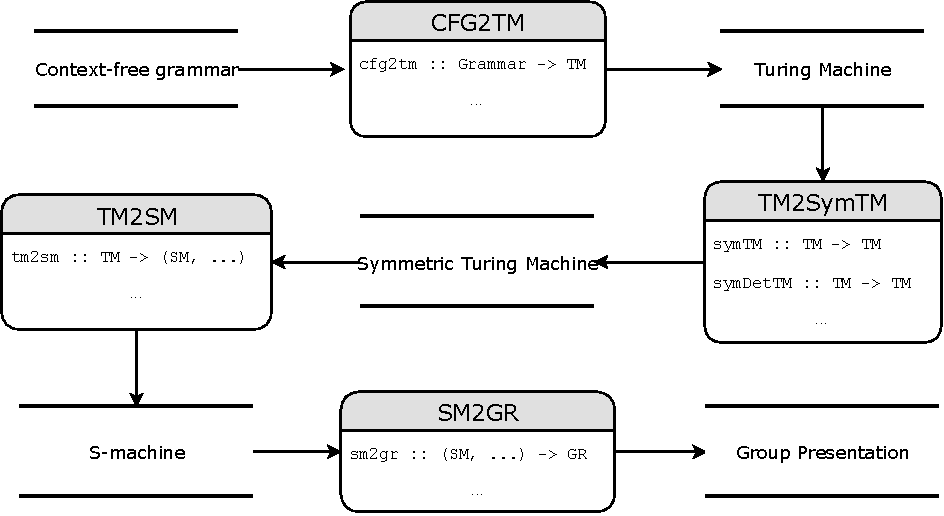
\includegraphics[width=\linewidth]{pics/diplomaSmallUML.pdf}
  \caption{Архитектура реализации}
  \label{fig:arch}
\end{figure}

\subsection{Типы данных, реализованные в работе}
В данной работе были использованы типы данных языка Haskell. На рис. \ref{fig:types} изображен листинг кода с типами данных, которые представляют грамматики, машины Тьюринга, S-машины и представления групп соответственно. Стоит отметить, что типы данных были намеренно описаны так же, как и в определениях соответствующих понятий. Это было сделано для поддержания максимальной схожести со статьей. 

\begin{figure}[H]
\begin{minted}[]{haskell}
-- грамматика
newtype Grammar = Grammar 
                        (Set Nonterminal, -- множество нетерминалов
                        Set Terminal, -- множество терминалов
                        Set Relation, -- множество правил
                        StartSymbol) -- стартовый нетерминал
-- машина Тьюринга                        
newtype TM = TM 
                (InputAlphabet, -- входной алфавит
                [TapeAlphabet], -- алфавиты лент
                MultiTapeStates, -- множества состояний лент
                Commands, -- множество команд
                StartStates, -- вектор стартовых состояний
                AccessStates) -- вектор конечных состояний
-- S-машина                
data SM =  SM 
            {yn :: [[Y]], -- алфавиты лент
            qn :: [Set State], -- множество состояний лент
            srs :: [SRule]} -- правила
-- представление группы        
newtype GR =  GR 
                (Set A, -- множество порождающих
                Set GrRelation) -- множество отношений
\end{minted}
\caption{Осноные типы данных, используемые в работе}
\label{fig:types}
\end{figure}

\subsection{Построение машины Тьюринга по контекстно-свободной грамматике}
Первая часть алгоритма не связана со статьей, рассмотренной в предыдущем разделе, 
и направлена на то, чтобы построить машину Тьюринга по контекстно-свободной грамматике 
с эквивалентным распознающимся языком.
Чтобы достичь этого, был реализован автомат с магазинной памятью в терминах машины Тьюринга, 
которая была представлена в определении~\ref{tm}, с некоторыми 
расширениями для обеспечения детерминированности машины там, где это возможно.

Алгоритм принимает формальную грамматику в нормальной форме Хомского в качестве входных данных.
Это необходимо для облегчения реализации и делается заранее.

Как было упомянуто ранее в теореме~\ref{thmpda}, автомат с магазинной памятью позволяет нам распознавать контекстно-свободные языки и, в конце концов, с машиной Тьюринга, распознающей контекстно-свободные языки, возможно построить представление групп для контекстно-свободных языков
(см. теорему~\ref{basethm}). 
Таким образом, в рамках этой работы не разработаны распознаватели для более 
широких классов языков, которые в общем случае машина Тьюринга может распознавать 
(например, рекурсивно перечислимые,булевы, конъюнктивные), поэтому для них в настоящее время нельзя 
построить представление группы. Однако для классов языков, являющихся подклассом 
контекстно-свободных, это возможно. 

Преобразование контекстной-свободной грамматики в машину Тьюринга реализовано в модуле \textbf{CFG2TM} алгоритма (см. рис. \ref{fig:cfg2tm}) и может быть запущено с помощью функции \textit{cfg2tm}. 

\begin{figure}[H]
\centering
  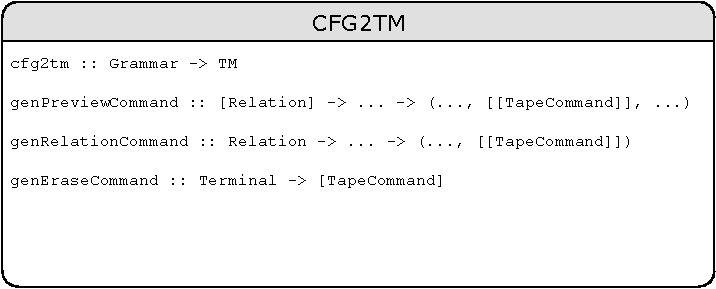
\includegraphics[width=\linewidth]{pics/cfg2tm.pdf}
  \caption{Схема модуля преобразования контекстно-свободной грамматики в машину Тьюринга}
  \label{fig:cfg2tm}
\end{figure}

Итак, машина Тьюринга, распознающая контекстно-свободные языки, состоит из двух лент: первая
лента для входного алфавита, вторая для имитации стека магазинного автомата. 
$\overline{s_1} = (q_0^1, q_0^2)$, $\overline{s_0} = (q_1^1, q_2^2)$ --- вектора начальных и конечных
состояний соответственно. 

Первая команда машины Тьюринга помещает на вторую ленту стартовый нетерминал:
$$\begin{array}{lcl}
    q_0^1 \omega \to q_0^1 \omega \\
    q_0^2 \omega \to S q_1^2 \omega 
\end{array}$$

Также вводится принимающая команда, которая переводит текущий вектор состояний машины Тьюринга в вектор конечных состояний, если на лентах пусто, то есть если слово было успешно принято:
$$\begin{array}{lcl}
    \alpha q_0^1 \omega \to \alpha q_1^1 \omega \\
    \alpha q_1^2 \omega \to \alpha q_2^2 \omega 
\end{array}$$

Следующие команды зависят от грамматики и разделяются на команды, производящие предпросмотр, команды, сгенерированные из правил грамматики, 
и команды, полученные из терминалов грамматики. Рассмотрим их по порядку.

Далее будет показано, что нам выгодно распознавать язык при возможности детерминированной машиной Тьюринга. Существуют грамматики, язык которых 
можно распознать детерминированной машиной Тьюринга, но по которым невозможно однозначно сразу определить какое правило нужно использовать. В качестве примера рассмотрим грамматику 
$$\begin{array}{lcl}
    S \to a S b \\
    S \to a b
\end{array}$$ 
Видя на ленте только литеру $a$, нельзя одним правилом определить, какое из этих двух правил нужно применить, так как первая литера  правой части правил одинакова. Поэтому в функции \textit{genPreviewCommand} генерируются правила, которые выполняют функцию предпросмотра на одну литеру вперед для определения, какое правило нужно применять следующим. Функция \textit{genPreviewCommand} на нашем примере генерирует следующие команды машины Тьюринга: 

$\begin{array}{lcl}
    a q_0^1 \to q_2^1 a \\
    S q_1^2 \omega \to S q_1^2 \omega 
\end{array}$,

$\begin{array}{lcl}
    a q_2^1 a \to a q_5^1 a \\
    S q_1^2 \omega \to S q_1^2 \omega 
\end{array}$,
$\begin{array}{lcl}
    b q_2^1 a \to b q_3^1 a \\
    S q_1^2 \omega \to S q_1^2 \omega 
\end{array}$,

$\begin{array}{lcl}
    q_5^1 a \to a q_5^1 \\
    S q_1^2 \omega \to S q_1^2 \omega 
\end{array}$,
$\begin{array}{lcl}
    q_3^1 a \to a q_3^1 \\
    S q_1^2 \omega \to S q_1^2 \omega 
\end{array}$,

$\begin{array}{lcl}
    a q_5^1 \omega \to a q_6^1 \omega \\
    S q_1^2 \omega \to S q_1^2 \omega 
\end{array}$,
$\begin{array}{lcl}
    a q_3^1 \omega \to a q_4^1 \omega \\
    S q_1^2 \omega \to S q_1^2 \omega 
\end{array}$.

Таким образом, если после литеры $a$ стоит снова литера $a$, то первая лента машины Тьюринга перейдет в состояние $q_6^1$, а если стоит литера $b$, то в состояние $q_4^1$, и так обеспечивается детерминированность машины Тьюринга, кодируя информацию о следующей литере состоянием. 

Далее рассмотрим какие команды машины Тьюринга генерирует функция \textit{genRelationCommand}.
Пусть в грамматике есть правило $A \to a A'$, тогда, чтобы симулировать это правило, машине Тьюринга
необходимо на второй ленте заменить $A$ на символы из правой части правила. Таким образом, из правила $A \to a A'$ получаются 
следующие команды машины Тьюринга: 

$\begin{array}{lcl}
    a q_0^1 \omega \to a q_0^1 \omega \\
    A q_1^2 \omega \to A' q_3^2 \omega 
\end{array}$,
$\begin{array}{lcl}
    q_0^1 \omega \to q_0^1 \omega \\
    q_3^2 \omega \to a q_4^2 \omega 
\end{array}$,
$\begin{array}{lcl}
    q_0^1 \omega \to q_0^1 \omega \\
    q_4^2 \omega \to q_1^2 \omega 
\end{array}$. 

Если же правая сторона правила состоит из одного символа, например, $A \to a$, то нет необходимости в генерации нового состояния для записи на стек, и можно обойтись следующей командой машины Тьюринга: 

$\begin{array}{lcl}
    a q_0^1 \omega \to a q_0^1 \omega \\
    A q_1^2 \omega \to a q_1^2 \omega 
\end{array}$. 

В случае, когда в грамматике есть правило, в котором правая часть является пустым словом, необходимо иначе генерировать команды машины Тьюринга. Например, рассмотрим грамматику 
$$\begin{array}{lcl}
    S \to \varepsilon \\
    S \to a S b
\end{array}$$
, тогда для правила $S \to \varepsilon$ функция \textit{genRelationCommand} сгенерирует следующие команды машины Тьюринга:

$\begin{array}{lcl}
    \alpha q_0^1 \omega \to \alpha q_0^1 \omega \\
    q_0^2 \omega \to S q_1^2 \omega 
\end{array}$,
$\begin{array}{lcl}
    \alpha q_0^1 \omega \to \alpha q_0^1 \omega \\
    S q_1^2 \omega \to q_1^2 \omega 
\end{array}$,
$\begin{array}{lcl}
    b q_0^1 \omega \to b q_0^1 \omega \\
    S q_1^2 \omega \to q_1^2 \omega 
\end{array}$.

Первая из них кладет на стек $S$ при стартовых состояниях и пустой входной ленте, вторая применяет правило, если входная лента пуста, а третья, если следующий символ на ленте $b$.  

Теперь рассмотрим команды машины Тьюринга, которые соответствуют терминалам грамматики и выполняют
функцию распознавания входного слова. Чтобы некоторый символ входного алфавита был распознан 
машиной Тьюринга, необходимо, чтобы он был наблюдаем на входной и стековой ленте. Считается, что
машина Тьюринга принимает некоторое слово, если после работы машины ее ленты пусты и она находится в
конечном состоянии. Таким образом, процесс распознавания символа заключается в стирании этого символа
с двух лент одновременно. Итак, любому терминалу $a$ соответствует следующая команда:

$\begin{array}{lcl}
    a q_0^1 \omega \to q_0^1 \omega \\
    a q_1^2 \omega \to q_1^2 \omega 
\end{array}$. 

Функция сопоставляющая каждому терминалу правило такого вида называется \textit{genEraseCommand}.

Таким образом, с помощью рассмотренных здесь функций производится преобразование контекстно-свободной грамматики в машину Тьюринга, распознающую язык этой грамматики. Кроме этого, в приложении \ref{app:grammar_example} приведен пример построения машины Тьюринга, используя данный алгоритм. 

\subsection{Симметризация машины Тьюринга}
Следующий шаг после построения машины Тьюринга --- это ее симметризация. Построение эквивалентной симметричной машины Тьюринга производится в модуле \textbf{TM2SymTM} (см. рис. \ref{fig:TM2SymTM}).

\begin{figure}[H]
\centering
  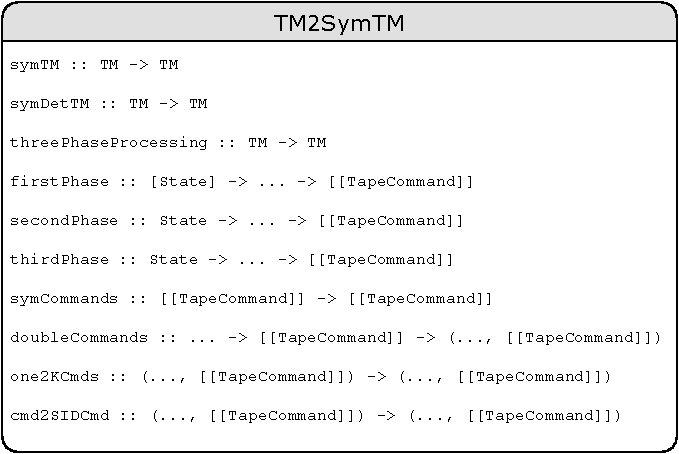
\includegraphics[width=\linewidth]{pics/TM2SymTM.pdf}
  \caption{Схема модуля симметризации машины Тьюринга}
  \label{fig:TM2SymTM}
\end{figure}

В ходе данной работы было реализовано два алгоритма симметризации машины Тьюринга. Один из них основан на теореме \ref{symthm}, которая доказана в статье \cite{Sapir}, а другой на теореме \ref{symDetTm}. Первый алгоритм может стоить эквивалентную симметричную машину Тьюринга как для детерминированной, так и для недетерминированной машины Тьюринга. Тут стоит отметить, что этот алгоритм в данной работе называется алгоритмом симметризации недетерминированной машины Тьюринга, так как детерминированные машины Тьюринга являются подклассом недетерминированных. Второй же алгоритм может давать на выходе эквивалентную симметричную машину Тьюринга, только если ему на вход была подана детерминированная машина Тьюринга, но при этом размер и сложность получившейся машины получается гораздо меньше, что будет показано далее.

Перейдем к рассмотрению этих двух алгоритмов.

\subsubsection{Алгоритм симметризации недетерминированной машины Тьюринга}
Весь алгоритм может быть запущен вместе с функцией \textit{symTM}, которая интегрирует функции, которые будут рассмотрены далее.

Итак, первая фаза алгоритма, как и в статье \cite{Sapir}, подразумевает построение новой машины Тьюринга $M'$, которая равна исходной за исключением добавленной $k+1$ ленты, где $k$ --- число лент у входной машины, такой, что ее алфавит состоит из команд входной машины Тьюринга. После чего, генерируются команды машины Тьюринга, которые недетерминированно заполняют $k+1$ ленту, единственное тут ограничение --- это то, что первая добавленная команда должна завершать вычисление исходной машины. Таким образом, после первой фазы на $k+1$ ленте машины Тьюринга $M'$ должна лежать последовательность команд исходной машины Тьюринга, где первая команда завершает ее вычисление (переводит вектор состояний в вектор конечных состояний). После этого происходит переход ко второй фазе. 

Вторая фаза заключается в том, что $M'$ пытается исполнить команды в том порядке, в котором они находятся на $k+1$ ленте. Для этого из команды исходной машины Тьюринга:
\begin{center}
    $\tau = \{ U_1 \to V_1, ... , U_k \to V_k \}$
\end{center}
строится команда $M'$:
\begin{center}
    $\tau' = \{ U_1 \to V_1, ... , U_k \to V_k, \tau q \to q \tau \}$
\end{center}
где $q$ --- состояние $M'$ на ленте $k+1$. 

Авторы утверждают, что после таких вычислений первая лента $M'$  опустеет, а $k+1$ справа будет наблюдать $\alpha$ только, если в течение первой фазы на $k+1$ ленту была записана последовательность команд исходной машины Тьюринга, которая приводит ее к конечным состояниям. 

После второй фазы $M'$ возвращает голову к $\omega$ на $k+1$ ленте и начинается третья фаза, которая заключается в очищении всех лент и переходе в вектор конечных состояний. 

Эти три фазы реализованы в функциях с соответствующими названиями \textit{firstPhase}, \textit{secondPhase}, \textit{thirdPhase}, а функция \textit{threePhaseProcessing} интегрирует их и строит $M'$ после этих трех фаз, в конце данной работы в приложении \ref{app:tm_example} можно увидеть результат работы этой функции на машине Тьюринга из одного правила. 

Как утверждается в \cite{symTM}, теперь можно из $M'$ построить эквивалентную симметричную машину Тьюринга добавлением в множество команд каждой команде ее обратную. В алгоритме это делает функция \textit{symCommands}. 

Таким образом, после этих шагов $M'$ удовлетворяет первым трем свойствам из теоремы \ref{symthm}, и остается преобразовать ее так, чтобы она удовлетворяла последним двум свойствам. 

Для достижения четвертого свойства происходит удваивание лент. Так для любой ленты $i$ появляется лента $i + 1/2$, такая что если изначально конфигурация ленты $i$: $\alpha u q v \omega$, то после удвоения конфигурации лент $i$ и $i+1/2$: $\alpha u q \omega$ и $\alpha \Bar{v} q \omega$ соответственно, где $u,v$ --- слова, $\Bar{v}$ --- слово $v$, записанное с права налево, $q$ состояние, которое далее переименовывается с целью достижения 5 свойства. В связи с этим необходимо заменить команды:
\begin{center}
    $\{ u_1 q_1 v_1 \to u_1' q_1' v_1',  ... , u_k q_k v_k \to u_k' q_k' v_k' \}$
\end{center}
на команды:
\begin{center}
    $\{ u_1 q_1 \omega \to u_1' q_1' \omega, \Bar{v_1} q_1 \omega \to \Bar{v'_1} q_1' \omega , ... , u_k q_k \omega \to u_k' q_k' \omega, \Bar{v_k} q_k \omega \to \Bar{v'_k} q_k' \omega \}$
\end{center}
Если $v$ в какой-то из команд равно $\omega$, то $\Bar{v} = \alpha$. Очевидно, что машина Тьюринга, которую преобразовали таким образом, будет распознавать такой же язык как и исходная машина Тьюринга. Эти преобразования реализованы в функции \textit{doubleCommands}. 

Следующее действие --- это разделение каждой команды на $2k$ команд, чтобы каждая новая команда затрагивала только одну ленту. Данная операция производится в функции \textit{one2KCmds}. Для этого генерируется для каждой команды множество уникальных состояний, чтобы поддерживать порядок вычисления. Таким образом получаются команды следующего вида: 
\begin{center}
    $\{ q_1 \omega \to q_1' \omega , ... , u_i q_i \omega \to u_i' q_i' \omega , ... \}$
\end{center}

Заметим, что если $u_i = \alpha$, то команда уже имеет вид (\ref{symType2}) так как $u_i'$ тоже равно $\alpha$, иначе требуется еще раз удвоить команду, чтобы они имели вид (\ref{symType1}) и это делает функция \textit{cmd2SIDCmd}:

\begin{center}
    $\{ q_1 \omega \to q_1'' \omega , ... , u_i q_i \omega \to q_i'' \omega , ... \}$
\end{center}

\begin{center}
    $\{ q_1'' \omega \to q_1' \omega , ... , q_i'' \omega \to u_i' q_i' \omega , ... \}$
\end{center}

Таким образом, производится построение машины Тьюринга, которая удовлетворяет 4 свойству теоремы \ref{symthm}. Чтобы удовлетворить 5 свойству, достаточно сгенерировать уникальные имена для состояний и литер, что в алгоритме происходит в процессе построения. 

\subsubsection{Алгоритм симметризации детерминированной машины Тьюринга}
Заметим, что первые три фазы алгоритма симметризации недетерминированной машины Тьюринга направленны на построение эквивалентной симметричной машины Тьюринга и, если у нас есть альтернативный вариант ее построения, эти действия можно не производить. 

Как было написано выше, согласно теореме \ref{symDetTm} можно симметризовать детерминированную машину Тьюринга, просто добавив в множество команд каждой команде ее обратную, и этого достаточно для построения эквивалентной симметричной машины Тьюринга. Но свойства 4 и 5 теоремы \ref{symthm} все равно нужно обеспечить в симметричной машине, чтобы перейти на следующий шаг построения представления группы. 
Поэтому для успешного построения эквивалентной симметричной машины Тьюринга по детерминированной машине Тьюринга достаточно выполнить функцию \textit{symDetTM}, которая интегрирует в себе функции \textit{doubleCommands}, \textit{one2KCmds}, \textit{cmd2SIDCmd} и \textit{symCommands}, рассмотренные выше и гарантирующие выполнение свойств 4 и 5. Кроме того, в приложении \ref{app:tm_example} можно увидеть пример работы алгоритма.

\subsection{Построение S-машины по симметричной машине Тьюринга}
В этом разделе будет рассмотрен алгоритм построения S-машины, симулирующей симметричную машину Тьюринга и в некотором смысле сохраняющей язык, распознаваемый этой машиной Тьюринга. Модуль, в котором реализованы функции, необходимые для построения, называется \textbf{TM2SM}, и его схема представлена на рис. \ref{fig:TM2SM}. Функция, производящая построение S-машины, называется \textit{tm2sm}, далее рассмотрим функции, суперпозицией которых она является.

\begin{figure}[H]
\centering
  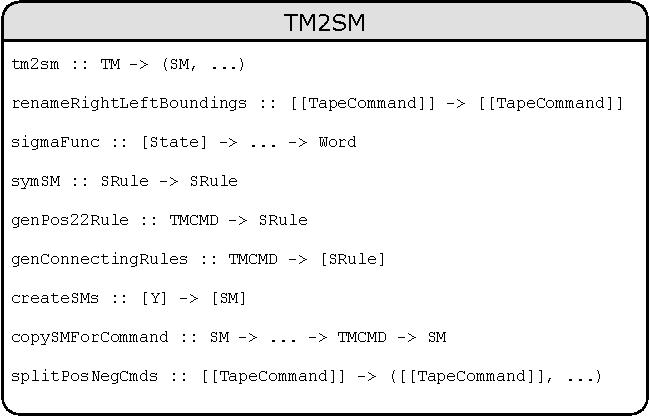
\includegraphics[width=\linewidth]{pics/TM2SM.pdf}
  \caption{Схема модуля построения S-машины, симулирующей машину Тьюринга}
  \label{fig:TM2SM}
\end{figure}

Как уже было написано в обзоре, перед непосредственно построением S-машины происходит переименования команд машины Тьюринга так, чтобы они имели одну из форм (\ref{21}, \ref{22}). Это действие в данной работе производит функция \textit{renameRightLeftBoundings}. Также в функции \textit{createSMs} строятся 11 вспомогательных S-машин: $S_1$, $S_2$, $S_3$, $S_4$, $S_5$, $S_6$, $S_7$, $S_8$, $S_9$, $S_{\alpha}$, $S_{\omega}$, и в функции \textit{genConnectingRules} генерируются S-правила, которые являются переходными между вспомогательными машинами. 

После этого каждой команде машины Тьюринга вида (\ref{21}) сопоставляется множество S-правил вспомогательных S-машин и переходных S-правил, а всем командам вида (\ref{22}) сопоставляется одно S-правило, которое не производит вычислений, но меняет состояние. Сопоставление происходит путем добавления к S-правилам метки принадлежности к определенной команде машины Тьюринга. 

Поиск команд вида (\ref{21}, \ref{22}) осуществляет функция \textit{splitPosNegCmds}, сопоставление множеств S-правил команде вида (\ref{21}) производит функция \textit{copySMForCommand}, а генерацию S-правила для команды вида (\ref{22}) функция \textit{genPos22Rule}.
Кроме этого реализована функция симметризации S-машины \textit{symSM} и функция $\sigma(C)$ (\textit{sigmaFunc}), значение которой было описано в обзоре.

Состояния получившейся S-машины --- это все состояния промаркированных вспомогательных S-машин, объединенные со всеми также промаркированными $E_i$ и $F_q$, которые были получены после переименования машин Тьюринга, где $i=1..k$ --- номер ленты, $q \in Q$ --- состояние машины Тьюринга.
Алфавит S-машины --- объединенные алфавиты вспомогательных S-машин с алфавитом машины Тьюринга. 

\subsection{Построение представления группы по S-машине}
Процесс построения представления группы по S-машине был подробно описан в теореме \ref{sm2gr}. В этом разделе покажем, какие функции производят это построение. 
\textbf{SM2GR} --- модуль, в котором содержаться эти функции (см. рис. \ref{fig:SM2GR}).

\begin{figure}[H]
\centering
  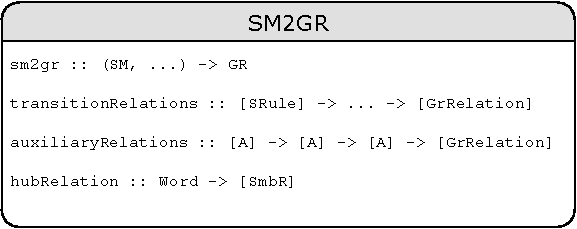
\includegraphics[width=\linewidth]{pics/SM2GR.pdf}
  \caption{Схема модуля построения представления группы по S-машине}
  \label{fig:SM2GR}
\end{figure}

Переходные вспомогательные отношения и отношение хаба генерируются в функциях \textit{transitionRelations}, \textit{auxiliaryRelations} и \textit{hubRelation} соответственно. Образующие представления группы генерируются в функции \textit{sm2gr}, которая, кроме этого, объединяет все отношения.

\subsection{Вспомогательные инструменты}
В этом разделе будут описаны дополнительные модули приложения, разрабатываемого в рамках данной работы, которые были написаны, во-первых, с целью облегчить восприятие и, во-вторых, для проверки эквивалентности преобразований в контексте сохранения распознаваемого языка при переходах от машины к машине. 

Для первого были разработаны модули, которые генерируют код LaTeX, с возможностью его генерации для отображения грамматик, машин Тьюринга, конфигураций машин Тьюринга, S-машин. 
Для такой генерации использовалась библиотека HaTeX\footnote{HaTeX --- библиотека, реализующая синтаксис LaTeX и несколько полезных абстракций. 

Описание библиотеки: \url{https://hackage.haskell.org/package/HaTeX-3.22.2.0} 

Дата последнего посещения: 14.05.20}. 
Был создан класс ShowLaTeX и реализован для всех типов, которые необходимо было печатать в LaTeX. 
Таким образом, были реализованы модули на языке Haskell \textbf{GrammarPrinter}, \textbf{TMPrinter}, \textbf{SMPrinter} и \textbf{ConfigPrinter}, в которых реализован класс ShowLaTeX для типов \textit{Grammar}, \textit{TM}, \textit{SM} и \textit{Configs} соответственно. Примеры такой генерации можно наблюдать в приложениях \ref{app:grammar_example} и \ref{app:tm_example}.

Для второго были написаны модули, которые интерпретируют отдельно машины Тьюринга и S-машины на заданных входных данных, общая концепция которых заключается в обходе дерева конфигураций в ширину с остановкой алгоритма в случае нахождения в фронте конечной конфигурации. Так, при обходе в ширину к каждой конфигурации из фронта необходимо применить команды машины Тьюринга или S-правила, которые возможно применить к данной конфигурации, а получившиеся конфигурации после применения добавить в множество фронта. 

Такой обход в ширину хорошо работает в случае с машиной Тьюринга, а в интерпретаторе S-машины из-за ее сильной недетерминированности было также использовано множество, в котором хранятся пройденные конфигурации. Если после применения правила получившаяся конфигурация уже есть в этом множестве, то такая конфигурация не добавляется в фронт. Таким образом, исключается возможность возвращения к уже пройденным конфигурациям, что облегчает поиск конечной конфигурации.  

Результатом работы интерпретаторов является история пройденных конфигураций, которые привели к конечной и из которых при необходимости можно сгенерировать LaTeX. 

Функции для интерпретации машины Тьюринга содержатся в модуле \textbf{TMInterpreter}, где функция \textit{interpretTM} производит интерпретация. Аналогично модуль интерпретатора S-машины \textbf{SMInterpreter}, где \textit{interpretSM} производит интерпретацию. 
Кроме этого, в этом модуле присутствует функция \textit{getRestrictedGraph}, которая строит граф заданной высоты. После этого этот граф можно напечатать в dot-файл с помощью функции \textit{writeGraph} модуля \textbf{DotGraphWriter}, печатающей его с помощью библиотеки graphviz\footnote{graphviz --- пакет инструментов с открытым исходным кодом для визуализации графов. 

Описание библиотеки: \url{https://hackage.haskell.org/package/graphviz}

Дата последнего посещения: 14.05.20}. 

Кроме этого, были реализованы модули, которые печатают представление группы в исходный файл математических пакетов GAP\footnote{GAP (Groups, Algorithms, Programming) --- программный пакет, система компьютерной алгебры с открытым исходным кодом и особым акцентом на вычислительную теорию групп.

Сайт пакета: \url{https://www.gap-system.org/}

Дата последнего посещения: 14.05.20} и Maple\footnote{Maple --- программный пакет, система компьютерной математики ориентированная на сложные математические вычисления, визуализацию данных и моделирование.

Сайт пакета: \url{https://www.maplesoft.com/products/Maple/}

Дата последнего посещения: 14.05.20}, для последующего анализа представления группы ими. 

Таким образом, у нас есть возможность наглядно продемонстрировать результат работы алгоритма и проверить совпадают ли распознаваемые языки после переходов. 

\section{Эксперименты}
В данном разделе приведены результаты работы цепочек алгоритмов построения представления группы из контекстно-свободных грамматик в нормальной форме Хомского с выводом численных размеров машин на всех шагах преобразования. 

Для оценки размера получившегося представления группы, запустили
алгоритмы с недетерминированной и детерминированной
симметризацией на трех грамматиках: грамматика из одного правила \eqref{eqonerule},
грамматика языка "a*" \eqref{eqastar} и однозначная грамматика языка Дика на одном типе скобок \eqref{eqdyck}.

\begin{multicols}{2}
\noindent
\centering
    \begin{align}
        \nonumber \\ S \to a \label{eqonerule}
    \end{align}
    \begin{align}
        S \to AS \nonumber \\
        S \to \epsilon \label{eqastar} \\
        A \to a \nonumber
    \end{align}
    \begin{align}
        S \to AC \nonumber \\
        S \to \epsilon \nonumber \\
        C \to SD \label{eqdyck} \\
        D \to BS \nonumber \\
        A \to a \nonumber \\
        B \to b \nonumber
    \end{align}
\end{multicols}

Таблица \ref{tab:countndtm} демонстрирует размеры каждого из множеств наших алгебраических типов, построенных в процессе работы алгоритма с недетерминированной симметризацией машины Тьюринга. По ней очевидно, что был получен алгоритм, который даже на простых исходных данных строит довольно большое представление группы. Итак, грамматика только из одного правила превращается в около 90 тысяч групповых отношений и 56 тысяч образующих. 

\begin{table}[H]
\centering
\begin{tabular}{|c|
c|c|c|
c|c|c|c|}
\hline
&
\multicolumn{3}{|c|}{\textbf{Grammar}}&
\multicolumn{4}{|c|}{\textbf{TM}}\\
\cline{2-8}
&$\Sigma$&$N$&$R$
&$X$&$\Gamma$&$Q$&$\Theta$\\
\hline
1 rule
&1&1&1
&1&3&5&4\\
\hline
$a^*$
&1&2&3
&1&4&7&9\\
\hline
Dyck
&2&4&6
&2&8&11&19\\
\hline
\end{tabular}
\begin{tabular}{
|c|c|c|c|
c|c|c|
c|c|}
\hline
\multicolumn{4}{|c|}{\textbf{SymTM}}&
\multicolumn{3}{|c|}{\textbf{SM}}&
\multicolumn{2}{|c|}{\textbf{G}}\\
\cline{1-9}
$X$&$\Gamma$&$Q$&$\Theta$
&$Y$&$Q$&$\Theta$
&$A$&$R$\\
\hline
1&14&270&206
&14&88246&2363
&89508&56187\\
\hline
1&26&547&434
&26&344118&5741
&347370&204903\\
\hline
2&54&1131&900
&54&1469136&15064
&1478859&957619\\
\hline
\end{tabular}
\caption{Мощности множеств машин при использовании алгоритма симметризации недетерминированных машин Тьюринга}
\label{tab:countndtm}
\end{table}


Но анализируя эту таблицу, можно заметить, что основной рост размеров происходит на этапах симметризации машины Тьюринга и преобразования симметричной машины Тьюринга в S-машину. Поэтому, чтобы уменьшить размер симметричной машины Тьюринга, был реализован алгоритм симметризации детерминированной машины Тьюринга, который также рассмотрен выше. Таблица \ref{tab:countdtm} демонстрирует результаты его работы. 

\begin{table}[H]
\centering
\begin{tabular}{|c|
c|c|c|
c|c|c|c|}
\hline
&
\multicolumn{3}{|c|}{\textbf{Grammar}}&
\multicolumn{4}{|c|}{\textbf{TM}}\\
\cline{2-8}
&$\Sigma$&$N$&$R$
&$X$&$\Gamma$&$Q$&$\Theta$\\
\hline
1 rule
&1&1&1
&1&3&5&4\\
\hline
$a^*$
&1&2&3
&1&4&7&9\\
\hline
Dyck
&2&4&6
&2&8&11&19\\
\hline
\end{tabular}
\begin{tabular}{
|c|c|c|c|
c|c|c|
c|c|}
\hline
\multicolumn{4}{|c|}{\textbf{SymTM}}&
\multicolumn{3}{|c|}{\textbf{SM}}&
\multicolumn{2}{|c|}{\textbf{G}}\\
\cline{1-9}
$X$&$\Gamma$&$Q$&$\Theta$
&$Y$&$Q$&$\Theta$
&$A$&$R$\\
\hline
1&6&39&34
&6&6058&501
&6410&7637\\
\hline
1&8&73&72
&8&15888&1024
&16565&17657\\
\hline
2&16&161&158
&16&67754&2837
&69772&71533\\
\hline
\end{tabular}
\caption{Мощности множеств машин при использовании алгоритма симметризации детерминированных машин Тьюринга}
\label{tab:countdtm}
\end{table}

Заметим, что действительно использование этого алгоритма уменьшило в несколько раз размер симметричной машины Тюринга, S-машины и представления группы по сравнению с использованием алгоритма симметризации недетерминированных машин Тьюринга. Понятно, что чем меньше представление группы, тем проще найти слова, которые равны групповой единице. Из этого можно сделать вывод, что в случае детерминированных грамматик, нужно использовать симметризацию для детерминированных машин.

Также были предприняты попытки проверить на равенство единице некоторые слова из полученных представлений групп с помощью математических пакетов GAP и Maple. К сожалению, из-за сложности вычислений математические пакеты, с которыми проводились эксперименты, не завершали свою работу в приемлемое время.

\section*{Заключение}
В ходе выполнения данной работы были достигнуты следующие результаты:
\begin{enumerate}
    \item Реализован алгоритм преобразования контекстно-свободной грамматики в машину Тьюринга.
    \item Разработан алгоритм построения представления группы по машине Тьюринга.
    \item Разработаны интерпретаторы машины Тьюринга и S-машины.
    \item Проведен ряд экспериментов.
\end{enumerate}

Так как описанное решение на данный момент не имеет своего применения, существует необходимость в его улучшении, а именно, если хочется получить представление группы удовлетворительных размеров, то в дальнейшей работе необходимо узнать, как более оптимальным образом преобразовать симметричные машины Тьюринга в S-машины. 

Мы можем утверждать, что возможно найти более оптимальный алгоритм построения S-машины по симметричной машине Тьюринга по ряду причин.
Во-первых, потому что существуют альтернативные способы построения S-машины по симметричной машине Тьюринга \cite{SpaceFunc}.
Во-вторых, так как по некоторым языкам можно построить представление группы, например, для языка $L = \{a\}$ можно построить представление группы и отношение из теоремы \ref{basethm}, такое что 
$$G=\langle k_1, k_2, a ~|~ k_1 a k_2 = 1 \rangle$$ 
и $K(a) = k_1 a k_2$. Понятно, что такое построение работает только для конечных языков, но это наталкивает на мысль, что, возможно, существует более простое построение и в общем случае. 

Кроме этого, актуальным остается вопрос интерпретации представления группы, так как существующие математические пакеты не смогли справится с этой задачей. 

\begin{appendices}

\section{Преобразование грамматики} \label{app:grammar_example}
В этом разделе приведен пример работы вышеизложенного алгоритма преобразования элементарной грамматики в машину Тьюринга с последующей ее интерпретацией.

Из следующей грамматики, состоящей из одного правила:
\subfile{examples/1rg.tex}

Была получена следующая машина Тьюринга с помощью алгоритма реализованного в рамках данной работы:
\subfile{examples/1rgtm.tex}

После чего проинтерпретировали получишуюся машину Тьюринга на входной строке $a$ и получили историю изменения конфигураций:
\subfile{examples/1rgtmconfg.tex}

\section{Преобразование машины Тьюринга} \label{app:tm_example}
В данном разделе рассмотрен пример работы трех фаз алгоритма симметризации недетерминированных машин Тьюринга, а именно функции \textit{threePhaseProcessing}, и также алгоритма симметризации детерминированной машины Тьюринга.

Из машины Тьюринга, содержащей одно правило и принимающей язык из одного слова $a$: 
\subfile{examples/1rtm.tex}

После трех фаз симметризации алгоритмом для недетерминированных машин получаем симметричную машину Тьюринга, которая не удовлетворяет 4 свойству теоремы \ref{symthm}: 
\subfile{examples/1rtm3phase.tex}

А применяя алгоритм симметризации детерминированной машины Тьюринга к той же элементарной машине, получаем симметричную машину Тьюринга:
\subfile{examples/1rtmsym.tex}

\end{appendices}

\setmonofont[Mapping=tex-text]{CMU Typewriter Text}
\bibliographystyle{ugost2008ls}
\bibliography{diploma.bib}
\end{document}
